\section{Theory}

In the following section, equations and algorithms used to model the behavior of
a symmetric ideal gas centrifuge cascade from individual centrifuge properties
are described. Details will also be provided to model centrifuge behavior
when fed with a different feed enrichment than designed.

\subsection{Centrifuge properties}

\subsubsection{Separative power}

\paragraph{R\"aetz equation}

As described by Glaser in \cite{glaser.2008}, the separative power of a single centrifuge can be express as an analytical solution \cite{raetz.phd} of the
differential equation for the gas centrifuge:

\begin{eqnarray}
    \label{eq:raetz}
    \delta U(L,F,\theta,Z_{p}) &= &\frac{1}{2}
            F\theta(1 - \theta)
            \left(\frac{\Delta M}{2 RT}v_{a}^{2}\right)^{2}
            \left(\frac{r_{2}}{a}\right)^{4}
            \left[1 - \left(\frac{r_{1}}{r_{2}}\right)^{2}\right]^{2}
            \label{eq_raetz}\\
        &&
            \left[
                \left(\frac{1+L/F}{\theta}\right)
                (1- exp[ - A_{P}(L,F,\theta)Z_{p}])  \nonumber  \right. \\
        &&~~ + \left.\left(\frac{L/F}{1 - \theta}\right)
                (1 - exp[ -A_{W}(L,F,\theta)(Z - Z_{p}])\right]^{2}, \nonumber
                \\
    \textrm{with~ ~ ~ ~ ~}
        A_{P} &= &\frac{2\pi D\rho }{ ln(r_{2}/r_{1}) }
                 \frac{ 1 }{ F }
                 \frac{ 1-\theta }{(1+L/F)(1-\theta+L/F) }\\
        A_{W} &= &\frac{2\pi D\rho }{ ln(r_{2}/r_{1}) }
                 \frac{ 1 }{ F }
                 \frac{ 1-\theta }{ (L/F)(1-\theta+L/F) }
\end{eqnarray}

In this equation, the parameters of average gas temperature, $T$, peripheral speed,
$v_a$, height, $h$, diameter, $d$, pressure ratio, $x$, feed flow rate, $F$,
counter-current flow ratio, $L/F$, are intrinsic to the centrifuge design.
To match the cascade design describe in \cite{glaser.2008} and \cite{walker.2017},
P1-type centrifuge properties have been chosen (Table \ref{tab:centrifuges}).

\begin{table}[htb]
    \centering
    \caption{Summary of the centrifuge parameters.}
    \begin{tabular}{ccccccc}
        \toprule
        $T$[K] & $v$[m/s] & $h$[m] & $d$[m]   & $x$      & $F$[mg/s]  & $L/F$  \\
        \midrule
        320    & $320$    & $1.8$  & $0.105$  & $10^{3}$ & $13$       & 2   \\
        \bottomrule
    \end{tabular}
    \label{tab:centrifuges}
\end{table}

The variable $Z_p$ is the rectifier length, or the location of the feed point,
and has an optimal axial location as defined by \cite{raetz.phd}:

\begin{equation}
    Z_p = \frac{(1-\theta)(1+L/F)}{1-\theta+L/F}Z
\end{equation}

This optimizes the recitifer length based on the cut, $\theta$, which is an expression
of the fraction of the centrifuge feed that is output as product, and the counter-current
flow, $L/F$. In practice, this value is a design parameter that is defined in the model
during the design of the centrifuge cascade.

The parameters $r_1$ and $r_2$ are the separation radii of the enriched material
(here ${}^{235}\mathrm{U}$ vs. ${}^{238}\mathrm{U}$), $r_1$ being the withdrawal
radius for the lighter isotope and $r_2$ for the heavier isotope. R\"aetz's
two-shell model looks for optimal values between these two, as described by
the hydrodynamic equations. The radii ratio is optimized using the following relationship:

\begin{equation}
    \max \left\{ \left[1-\left(\frac{r_1}{r_2}\right)^2 \right]^2 \times \left[ \ln \left(\frac{r_2}{r_1} \right) \right]^{-1} \right\}
\end{equation}

This ratio can further be constrained by approximating $r_2$ as being very close
to the inner centrifuge wall with radius $a$:

\begin{equation}
    \left(\frac{r_1}{r_2}\right) \approx \left(\frac{r_1}{a}\right) = \sqrt{1 - \frac{2RT}{M}(\ln x)\frac{1}{v_{a}^{2}}}
\end{equation}
 
Here the gas constants are molar mass, $M$, temperature $T$, universal gas constant, $R$,
and the pressure ratio, $x$ (typically $1000:1$) \cite{}. %needs citation?
This relationship is valid when $v_a > 380 \frac{\mathrm{m}}{\mathrm{s}}$.
Otherwise, the relationship can be approximated $\{\frac{r_1}{r_2} \approx 0.534 \mid v_a \leq 380 \frac{\mathrm{m}}{\mathrm{s}}\}$.
In order to decompose the ratio into each individual radius, knowledge on one
of them is required. Glaser \cite{glaser.2008} states that $r_2$ typically ranges
from $96\%$ to $99\%$ the value of the inner centrifuge wall radius $a$. The exact
behavior of $r_2$ between these two values in operational conditions is unknown,
but a linear approximation can be made. It is assumed that $r_2$ is always at
the midpoint of these two extremes (i.e. $r_2 = 0.975 a$). Then, $r_1$ can be
found by simply multiplying this value by the ratio.

With this, all parameters of the separative power equation \ref{eq:raetz} are
defined and a value can be calculated. Separative power, $\delta U$, has units similar to the feed flow, that of $[mg/s]$.

\paragraph{First principle}

It can be shown \cite{avery} that the separative power of a single centrifuge can be
derived from first principles and expressed as a function of the feed-to-product enrichment factor, $\alpha$, the cut, $\theta$, and the feed rate, $F$:
%I think we should replicate at least some of that here

\begin{equation} \label{eq_alpha_principle}
    \delta U = \frac{F}{2}\frac{\theta}{1-\theta}(\alpha-1)^{2}
\end{equation}

\subsection{Centrifuges basic properties and definition}

The outputs of a centrifuge relative to its input can be described with ratios
of the abundance ($R = \frac{N}{1-N}$) where the feed, product, and tail enrichment $N, N', N''$ respectively. Enrichment factors of $\alpha$ (feed-to-product),
$\beta$ (feed-to-tail), and $\gamma$ (tail-to-product) can then be defined:

\begin{subequations}
    \label{eq_alphabeta}
    \begin{equation} \label{eq_alpha_def}
        \alpha = \frac{1-N}{N}\frac{N'}{1-N'}
    \end{equation}
    \begin{equation}\label{eq_beta-def}
        \beta = \frac{1-N''}{N''}\frac{N}{1-N}
    \end{equation}
    \begin{equation}\label{eq_gamma-def}
        \gamma = \alpha \, \beta
    \end{equation}
\end{subequations}


\subsection{Cascade Design}
\subsubsection{Symmetric Cascade}

A symmetric cascade is a cascade where a stage is fed using the tail, $T$, of the next stage and the product, $P$, of the previous one. The the cascade feeding stage, $F_{i}$ flow, with external feed, $F_{ext}$, is given by:

\begin{equation}
    F_{i} = T_{i+1} + P_{i-1} ~(+ F_{ext})
\end{equation}

\subsubsection{Symmetric Ideal Cascade}
This model constructs cascades as symmetrical and ideal, with no losses in
separative work. This means that the tail assay of the next stage ($N''_{i+1}$)
is the product assay of the previous stage ($N'_{i-1}$), which can be
expressed as:

\begin{equation}
    \forall i~ N_{i} = N'_{i-1} = N''_{i+1}~ ~\Leftrightarrow~ ~\forall (i,j)~
    \alpha_{i} = \beta_{j}
\end{equation}



\subsection{Building the cascade}

Designing a symmetric ideal cascade beings with the feeding
stage. As all the enrichment factors are equal across all the cascade, the
feeding stage is used to determine all subsequent stages.
The feed assay of the feeding stage, $N_{0}$, is fixed by the external feed assay
provided as an input.

From equation \eqref{eq_raetz} and \eqref{eq_alpha_principle} it is possible to
express the feed-to-product enrichment factor $\alpha$ as a function of the feed rate $F$, the separative performance
$\delta U$ (a function of $\theta$), and the cut $\theta$:

\begin{equation} \label{eq_alpha}
    \alpha = \sqrt{\frac{2\delta U(\theta)}{F} \frac{1-\theta}{\theta}} + 1
\end{equation}


From equations \eqref{eq_alphabeta}, the product assay can be expressed as:

\begin{equation}\label{eq_product_assay}
    N' = \frac{\alpha \frac{N}{1-N}}{1+\alpha \frac{N}{1-N}} = \frac{\alpha R}{1 + \alpha R}
\end {equation}


Then, from mass conservation, $N = \theta N' + (1-\theta)N''$ and equation
\eqref{eq_product_assay}, it is possible to express the feed-to-tail enrichment factor $\beta$ as a function of only the feed abundance, $R$, the cut $\theta$, and the feed-to-product enrichment factor, $\alpha$:

\begin{subequations}
    \begin{equation}\label{eq_beta_interim}
        \beta = \left( 1 - \frac{N - \theta N'}{1-\theta} \right)
                        \left( \frac{R}{\frac{N - \theta N'}{1 - \theta}} \right)
    \end{equation}
    \begin{equation}\label{eq_beta}
        \beta =   R \left(\dfrac{1-\theta}
                        {\dfrac{R}{R+1}- \theta \dfrac{\alpha R}{1+\alpha R}} -1\right)
    \end{equation}
\end{subequations}

Finally from equation \eqref{eq_alpha} and \eqref{eq_beta} it is possible to
determine the cut, $\theta$, required to build an ideal cascade:

\begin{eqnarray}
    \theta_{i} = \dfrac{N_{i} - \dfrac{1}{1 + \beta/R_{i}}}{ \dfrac{\alpha R_{i}}{1 + \alpha R_{i}} -
           \dfrac{1}{1 + \beta/R_{i}}}
           \label{eq_theta}
\end{eqnarray}


To construct an ideal stage, a cut, $\theta$, must first be computed.
This is found iteratively, searching for the optimal cut value where $\alpha = \beta$
for given feed and centrifuge parameters. With a separative power calculated,
an $\alpha$ and $\beta$ value can be determined for an initial cut guess. This
model assumes that the ideal cut for a stage should be between 0.1 and 0.9. The
two enrichment factors are compared, and the higher or lower cut value is chosen
by which pair of factors are closer. A new cut is determined from the chosen
factors, a new separative power is computed, and new $\alpha$ and $\beta$ values
are compared. This process continues until, to some precision, the resulting
enrichment factors are approximately equal. As illustrated in Fig. \ref{fig_a_m_b},
for a given input feed assay, the ideal feeding stage typically has a $\theta$
value between 0.45 and 0.525 when $\alpha = \beta$.

\begin{figure}[h!] % replace 't' with 'b' to force it to be on the bottom
    \centering
    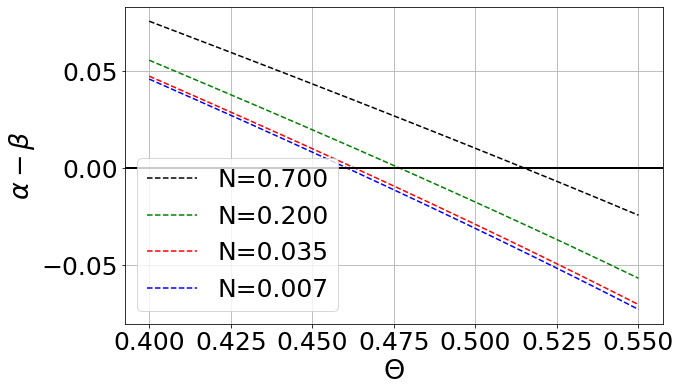
\includegraphics[scale=0.5]{alpha_minus_beta}
    \caption{Evolution of the difference between $\alpha$ and $\beta$ as a
    function of the cut value for different of feed assays, 0.007 (black),
    0.035 (red), 0.2 (green), 0.7 (black). }
    \label{fig_a_m_b}
\end{figure}

The number of machines required to construct a stage can then be computed using
equation \eqref{eq_alpha_principle} to solve for the centrifuge feed flow:

\begin{equation}\label{eq_cent_feed}
    F_c = \frac{2 \delta U}{(\alpha - 1)^2} \frac{M}{M_{238}} \frac{1-\theta}{\theta}
\end{equation}

Where the molar mass ratio $\frac{M}{M_{238}}$ accounts for the molar mass
differences between the feed gas, $UF_6$, and the individual uranium isotopes
being separated. The stage feed flow can then be divided by the individual
centrifuge feed flow, equation \eqref{eq_cent_feed}, to find the exact number of
machines needed for the ideal stage. In practice, this number is rounded up to
account for fractional machines required.


In a cascade, as the stage feed-to-product enrichment factor $\alpha_{i}$ and stage feed-to-tail enrichment factor $\beta_{i}$ remain constant, only the value of
the cut, $\theta_{i}$, changes across the different stages of a cascade.  This
algorithm assumes that the corresponding separative power $\delta U$ (not
re-computed) can be achieved with the chosen centrifuge design by tuning other
operational parameters such as the rotation speed, counter-current flow
ratio, etc.  Once $\theta_{i}$ is determined, it is possible to compute the
product and the tail assays.


The design of the ideal symmetric cascade is performed through 2 steps. First,
the configuration and number of stages is determined, adding stages with product assay $N'_i$ calculated using equation \ref{eq_product_assay}, until the
product assay of the final stage is greater than or equal to the product targeted assay. The stage tails assay $N''_i$ is calculated similarly, until it is less than or equal to the tails desired assay.  This determines the number of enriching and stripping stages as well as their enrichment properties ($N_{i}$, $N'_{i}$, $N''_{i}$,$\theta_{i}$).


The second step determines the relative flows at each stage, solving the linear
flow equation, \eqref{eq_flow}.
The cascade can then be populated with actual machines until the maximum number
of available machines is reached.

\begin{equation}
\resizebox{\linewidth}{!}{%
$\displaystyle
\setcounter{MaxMatrixCols}{20}
\begin{bmatrix}
     -1      & 1-\theta_{_{S+1}} & 0                 & ...  & 0            & 0            & 0             & 0             & 0             & ... & 0               & 0  & 0 \\
\theta_{_S}  & -1                & 1-\theta_{_{S+2}} & ...  & 0            & 0            & 0             & 0             & 0             & ... & 0               & 0  & 0 \\
             &                   &                   &      &              &              & ...           &               &               &     &                 &    &   \\
 0           & 0                 & 0                 & ...  & \theta_{_-2} & -1           & 1-\theta_{_0} & 0             & 0             & ... & 0               & 0  & 0 \\
 0           & 0                 & 0                 & ...  & 0            & \theta_{_-1} & -1            & 1-\theta_{_1} & 0             & ... & 0               & 0  & 0 \\
 0           & 0                 & 0                 & ...  & 0            & 0            & \theta_{_0}   & -1            & 1-\theta_{_2} & ... & 0               & 0  & 0 \\
             &                   &                   &      &              &              & ...           &               &               &     &                 &    &   \\
 0           & 0                 & 0                 & ...  & 0            & 0            & 0             & 0             & 0             & ... & \theta_{_{E-2}} & -1 & 1-\theta_{_E} \\
 0           & 0                 & 0                 & ...  & 0            & 0            & 0             & 0             & 0             & ... & 0               & \theta_{_{E-1}} & -1
 \end{bmatrix}
 \times
 \begin{bmatrix}
     F_{_{S}}   \\
     F_{_{S+1}} \\
     \cdots     \\
     F_{_{-1}}  \\
     F_{_{0} }  \\
     F_{_{1} }  \\
     \cdots     \\
     F_{_{E-1}} \\
     F_{_{E}}
 \end{bmatrix}
 =
 \begin{bmatrix}
     0      \\
     0      \\
     \cdots \\
     0      \\
     F      \\
     0      \\
     \cdots \\
     0      \\
     0
\end{bmatrix}
$}
%\caption{caption needed!}
\label{eq_flow}
\end{equation}



\subsection{Misuse models}

Little information is available about optimising an existing enrichment cascade
that is being fed with a feed enrichment that does not match the design
enrichment. Here, 3 different methods will be investigated.

The first method, A, assumes that no changes are being made to the cascade, i.e $\delta U$, $F$ and $\theta$ are fixed across all stages. The second method, B, assumes the cut value $\theta$ is re-tuned at each stage to maintain the ideal state of the cascade, while $\alpha$ and $\beta$ remain fixed. The last method, C, described in \cite{walker.2017} assumes the tails-to-product enrichment factor $\gamma$ and the cut $\theta$ remain constants
(eq. \eqref{eq_gamma-def}: $\gamma = \alpha\beta$). Model behaviors and
assumptions are summarized in Tab. \ref{tab:models}.

\begin{table}[htb]
\centering
  \caption{Summary of misuse model properties.}
\begin{tabular}{l|ccc}
\toprule

Model                &    A                 & B                  & C  \\
\midrule
Constant parameters  & $\alpha_i, \theta_i$ & $\alpha_i=\beta_i$ & $\gamma_i=\alpha_i\beta_i, \theta_i$       \\
Varying parameters   & $\beta_i$            & $\theta_i$         & $\alpha_i, \beta_i$                     \\
Assays determination & blended              & ideal              & blended                  \\
Flow                 & unchanged            & reduced            & unchanged       \\

\bottomrule
\end{tabular}
  \label{tab:models}
\end{table}

\subsubsection{Model A}

The tuning method A does not re-optimize $\theta_i$, keeping the same flow as the
ideal configuration. From equation \eqref{eq_alpha}, maintaining $\delta U$ and
$F$ while $\theta$ is unchanged implies $\alpha$ remains unchanged as well.
According to equation \eqref{eq_beta}, when $\alpha$ and $\theta$ are fixed, if
the feed assay ($N$) changes, $\beta$ will change accordingly.  This breaks the
ideal status of the cascade, i.e. $N_{i} \neq N'_{i-1} \neq N''_{i+1}$.


In order to compute the proper product and tails assay at each stage, the tail
and the product from the next and the previous stage respectively must be
blended in order to determine the correct stage feed assay. All feed assays are
iteratively updated, blending the proper product and tails, then using the
updated feed assay, the new product and tails assays are recomputed. This
process is repeated until the sum of the square difference in assays is smaller
than $10^{-8}$.  As the cut remains fixed at each stage, the flows do not need
to be recomputed.

This model assumes that it is possible to maintain the separative power of a
centrifuges, $\delta U$, for any feed assays $N$ while maintaining its cut
$\theta$ and feed flow $F$.

\subsubsection{Model B}

Using the second method, the cut value at each stage, $\theta_i$, is retuned in
order to maintain the $\alpha_i$ and $\beta_i$ at their original values
(equation \eqref{eq_theta}). Since the cascade remains ideal, the product and
tails assay at each stage can easily be determined using equations
\eqref{eq_alphabeta}.

As the cut values change, the relative flow rates between the different stages
are recomputed using equation \eqref{eq_flow}.  Under this model, the flow at
each stage of the original ideal cascade is assumed to be the maximum flow
allowed at that stage.  Therefore, all of the recomputed flow rates are scaled
together to ensure that no stage experiences a flow rate larger than that of
the original cascade.  Some stages may now experience flow rates much lower
than the original cascade.

%% The flow rates are determinted as
%% the largest flow rates allowed by the cascade design, number of centrifuges
%% limiting the flow at each stage.

This model assumes that it is possible to tune a centrifuge separative power
$\delta U$, for any feed assay $N$, cut $\theta$ and feed flow $F$, in order to
maintain its constant feed to product enrichment factor $\alpha$.




\subsubsection{Model C}
The last model assumes that the tails to product enrichment factor remains
constant regardless to the feed assays. To compute the response of the cascade
one need to determine $\alpha$ and $\beta$ such that their product and
$\theta$ remain fixed.
From equations \eqref{eq_alphabeta} and the assay conservation equation $N =
\theta N' + (1-\theta)N''$ it is possible to express the product, $N'$,
dependent on the feed assay $N$, $\gamma$, and the cut, $\theta$, as one
solution of the second order equation \eqref{eq_gamma_p}:

\begin{equation}\label{eq_gamma_p}
    \theta(\gamma-1)N'^2+((N+\theta)(\gamma-1)+1)N'-N\gamma = 0
\end{equation}


The only solution allowing product assay to range between 0 and 1 is the
following :

\begin{equation}\label{eq_model_b_sol}
    N' = \frac{N+\theta}{2\theta} +
         \frac{1 - \sqrt{\gamma^{2}(N-\theta)^{2}
                         + 2\gamma( N^{2} + N - \theta^{2} + \theta)
                         + (N + \theta + 1)^{2}}}
              {2\theta(\gamma - 1)}
\end{equation}

Once the product assay is known, one can trivially determine the tails assay,
$\alpha$ and $\beta$, using equations \eqref{eq_alphabeta} and mass
conservation.

Similar to model A, because the cut values remain constant, the flows do not
need to be recomputed and the correct assays, $\alpha$ and $\beta$, are
determined through iterative blending of the product assays of the previous
stage and the tails assay of the next stage using equation
\eqref{eq_model_b_sol}.

This model assumes that it is possible to tune the centrifuge separative power
$\delta U$ in order to maintain for any feed assay $N$ and its tails to product
enrichment factor $\gamma$ while maintaining its cut $\theta$ and feed flow $F$.

%The speed at which each models reach a threshold of $90\%$ enrichment is
%illustrated in Figure \ref{fig:model_comparison}. The production curve of
%enrichment for each model is shown. The step functions for each model represent
%the cascade configuration. Each step is one cascade in a chain of cascades and
%the shape of the curve for each model gives an indication of how quickly the model
%can reach the enrichment threshold. The main difference is that Model B reaches
%the threshold faster, whereas Models A and C reach a higher enrichment value.
%This highlights some of the immediate differences that would influence the choice
%of using each model in a breakout scenario.

%\begin{figure}[ht]
%    \centering
%    \includegraphics[scale=0.4]{ModelComparison}
%    \caption{The curve of resulting product assays for each model is plotted.
%    Since the feed assay of each cascade is fed into the next cascade in the
%    chain, a linear relationship between the product and feed assays is plotted
%    in black. The step function for each model represents the output of the
%    cascade chain (each step is a cascade). While there are four steps for each
%    model, Model B (green) reached the $90\%$ enrichment threshold before
%    Model A (red) or Model C (blue). However, in the same amount of steps, Models
%    A and C are able to achieve a higher enrichment percent than Model B.}
%    \label{fig:model_comparison}
%\end{figure}
